\section{Vine as a New Form of Expression}
As pointed out  by previous work \cite{redi20146}, micro-videos have been often called a ``new form of expression'' that goes beyond the traditional video medium.  Vine constraints (short length, limited editing tools) offer an unprecedented number of possibilities for creative visual artists. Tech journalists \footnote{\small \url{https://www.scientificamerican.com/article/why-micro-movies-so-popular-today/}} have indeed theorised that micro-videos cannot be even categorised as videos: their goal is to capture a single moment, thus making them ideally close to the photographic medium, or  \emph{``neither photo nor video but something in between, with artistic merits all its own''}. 

In this Section, we understand the novelty introduced  by the Vine platform in the media landscape using a computational approach. We consider 3 datasets of popular items from radically different platforms: Flickr (photography medium), Vine (micro-video medium) and Youtube (long video medium). We then compare these media over 3  dimensions: visual aesthetics, visual semantics and audio channel.
%
\vspace{3pt}\\\textbf{Datasets.} We consider the following datasets for platform comparison. (1) \emph{Photography medium:} we sample 1000 images from the MIR dataset (popular pictures from the Flickr stream) (2) \emph{Micro-Videos medium:} we consider our POP12K dataset (popular Vines) (3) \emph{Videos medium:}  we use the 447 viral YouTube videos from the CMU dataset.
%
\vspace{3pt}\\\textbf{Visual Aesthetics Comparison.} 
To compare the 3 platforms over the visual aesthetics dimension, we describe all items with the 18 computational aesthetics features from \textbf{SEC. BLA}. To obtain a description of the visual aesthetics trends for each medium, we aggregate the computed features at a platform-level. To do so, for each dataset, we compute the feature marginal probability distribution. This reflects the platforms' dominant visual aesthetics patterns (e.g. what are the common brightness values in YouTube videos? Or the distribution of Colorfulness in Vine?). To compare distributions across platforms (e.g. Rule of Thirds in Flickr VS Rule of Thirds in Vine), we then use symmetric Kullback-Lieber (KL) divergence, which reflects the distance of 2 probability distributions. The average of such KL divergence values  tells us how far platforms are in the visual aesthetics feature space. We report the results of this analysis in Fig. \ref{fig:comparisontable}: as expected, Vine videos show different visual aesthetic behaviour from both Flickr and Youtube, although more stylistically similar to long videos. 
\\
To understand why Vine is so different, we then look at the features with greater KL divergence across platforms. We notice that, in practice, Flickr aesthetic features reflect the behaviour of a "professional" medium, On the other side of the spectrum, micro-videos show patterns of less professional use, typical  of the  user-generated mobile-first Vine content. Youtube lies in the middle of such spectrum. More specifically, we notice the following (see Fig. \ref{fig:comparison_aesthetics}). (1) \emph{Colorfulness:}  Flickr photos tend to have a higher color diversity, while Vine and Youtube tend to have less saturated colors. (2) \emph{Exposure:}  Flickr pictures tend to have a good balance between Left and Right  pixel intensities, typical of high quality images; unlike Flickr, Youtube and Vine videos show unbalanced exposure. (3) ) \emph{Rule of Thirds:}  Flickr pictures tend to deviate from the standard rule of thirds, typical of professional, artistic pictures. On the other hand, the moving images of Vine and Youtube tend to stick to the Rule of Thirds rule (4) \emph{Sharpness} is probably one of the most important properties of high quality visual content. Due to its mobile-based nature, Vine videos tend to have almost no sharp pixels, while the professionally of Flickr photographers is clearly exposed by the higher percentage of sharp pixels.  
%
\vspace{3pt}\\\textbf{Visual Semantics Comparison.} 
To understand the semantic content depicted in Vine, Youtube and Flickr items, we use the deep learning-based object detectors from \textbf{CIT NEEDED}\cite{}. For each visual item, we retain the labels of top-5 objects detected. We then aggregate such information at a platform level by computing the multinomial distribution of the detected objects for all Flickr images, Vine videos, and Youtube videos.  Such distributions reflect  the frequency of visual objects in typical popular videos of each platform (e.g. how often does a cat appear in a YouTube video?). Again, we then use symmetric KL divergence to compare object distributions across platforms. From Fig. \ref{comparisontable}, we see that, in the object space, Youtube and Flickr are equally distant from Vine. By looking at element-wise differences across distributions, we then rank objects according to how different their frequencies are for the 3 platforms, and report results in Fig.\ref{fig:comparison_objects}. Vine can be clearly distinguished from the other 2 media due to the higher presence of objects related to celebrations, fun, entertainment (\emph{academic dress} ,\emph{wig},\emph{tv}, ,\emph{sunglasses}). Viral Youtube videos prefer popular subject such as kids (\emph{diaper}), cars, and  violent scenes (\emph{punching},\emph{neck brace}). Finally, Flickr pictures can be distinguished for the presence of visual concepts typical of suggestive sceneries ((\emph{lakeside}, (\emph{seashore}.)
%
\vspace{3pt}\\\textbf{Audio Channel Comparison.} 
The audio channel is as important as the visual channel for long videos. We want to understand here the role of audio in for Vine videos. For Youtube and Vine, we extract the audio features in \textbf{SEC. BLA}. Given the continuous nature of these features, we follow the same procedure used for  aesthetic feature analysis (per-feature symmetric KL divergence). In Fig. \ref{fig:comparisontable}, we see that in the audio space such media are far apart. This is due to the fact that, while the audio tracks of Youtube Videos are very diverse, and therefore follow almost-uniform distributions across different feature ranges, all audio tracks in Vine videos tend to have very similar patterns. In Vine, audio is mainly a weak complement to the visual counterpart: Vine videos can be fully consumed and understood without the audio channel, and they are often played in the mute mode. As a matter of fact, Vine videos tend to have few rythmical changes (low \emph{Onset Rate}) and low \emph{Roughness}. Also, overall, due to their less curated audios, Vine videos tend to be louder than Youtube videos (high \emph{Energy}), as shown in Fig. \ref{fig:comparison_audio}.

\begin{figure}[!htb]
\centering
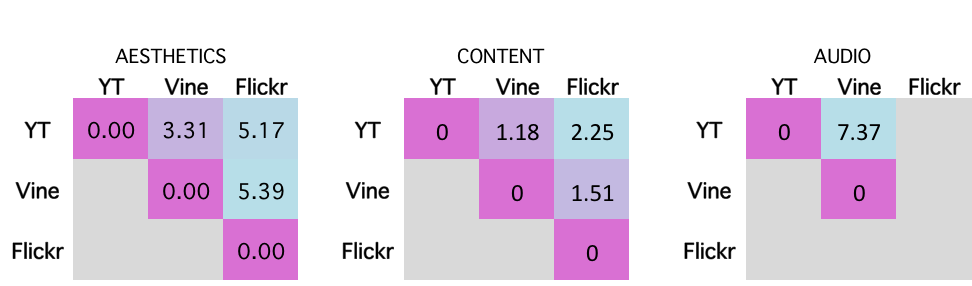
\includegraphics[width=\columnwidth]{plots/comparison/table}
\caption{\textsl{ Aggregated KL Divergences between platforms over all features for different feature groups.}}
\label{fig:comparisontable}
\end{figure}

\begin{figure}[!htb]
\centering
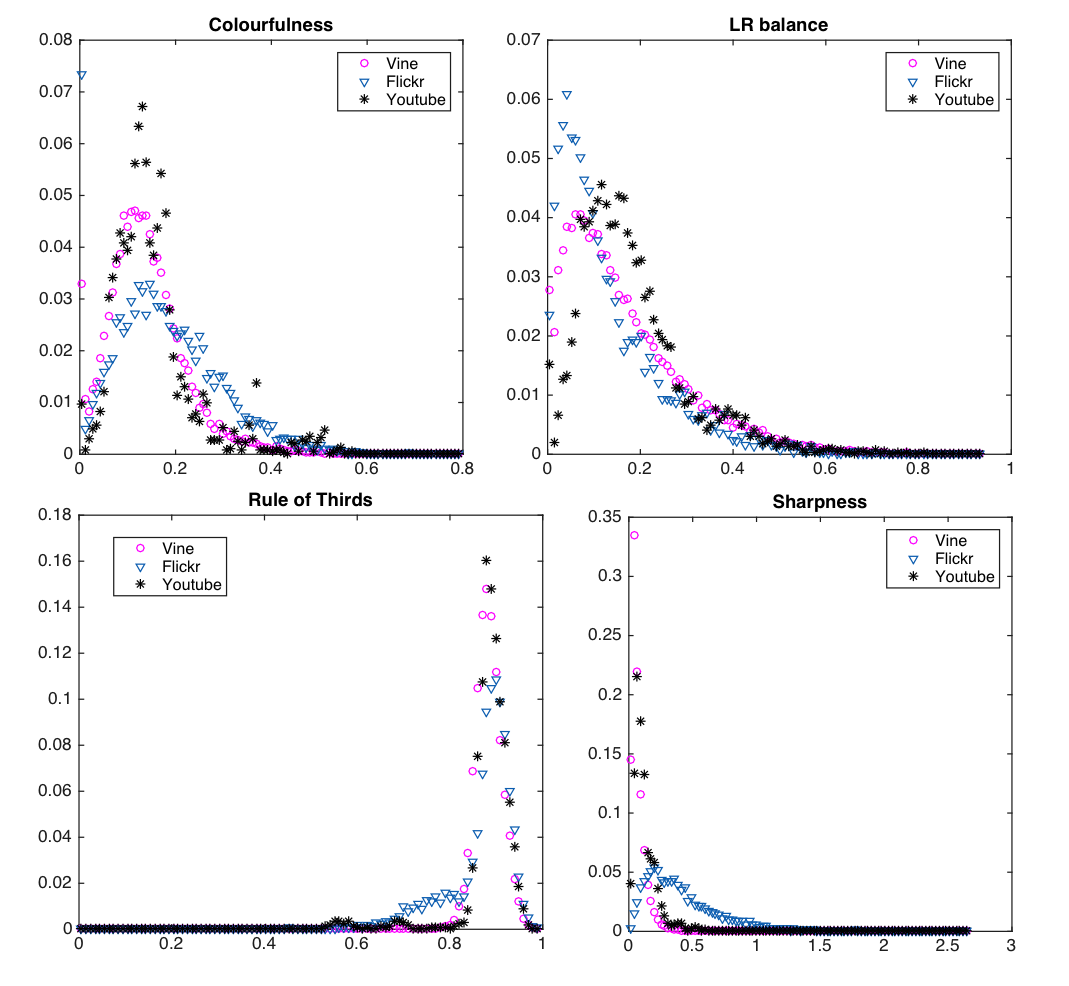
\includegraphics[width=\columnwidth]{plots/comparison/aesthetics}
\caption{\textsl{ Distributions of the most diverging aesthetic features across platforms.}}
\label{fig:comparison_aesthetics}
\end{figure}

\begin{figure}[!htb]
\centering
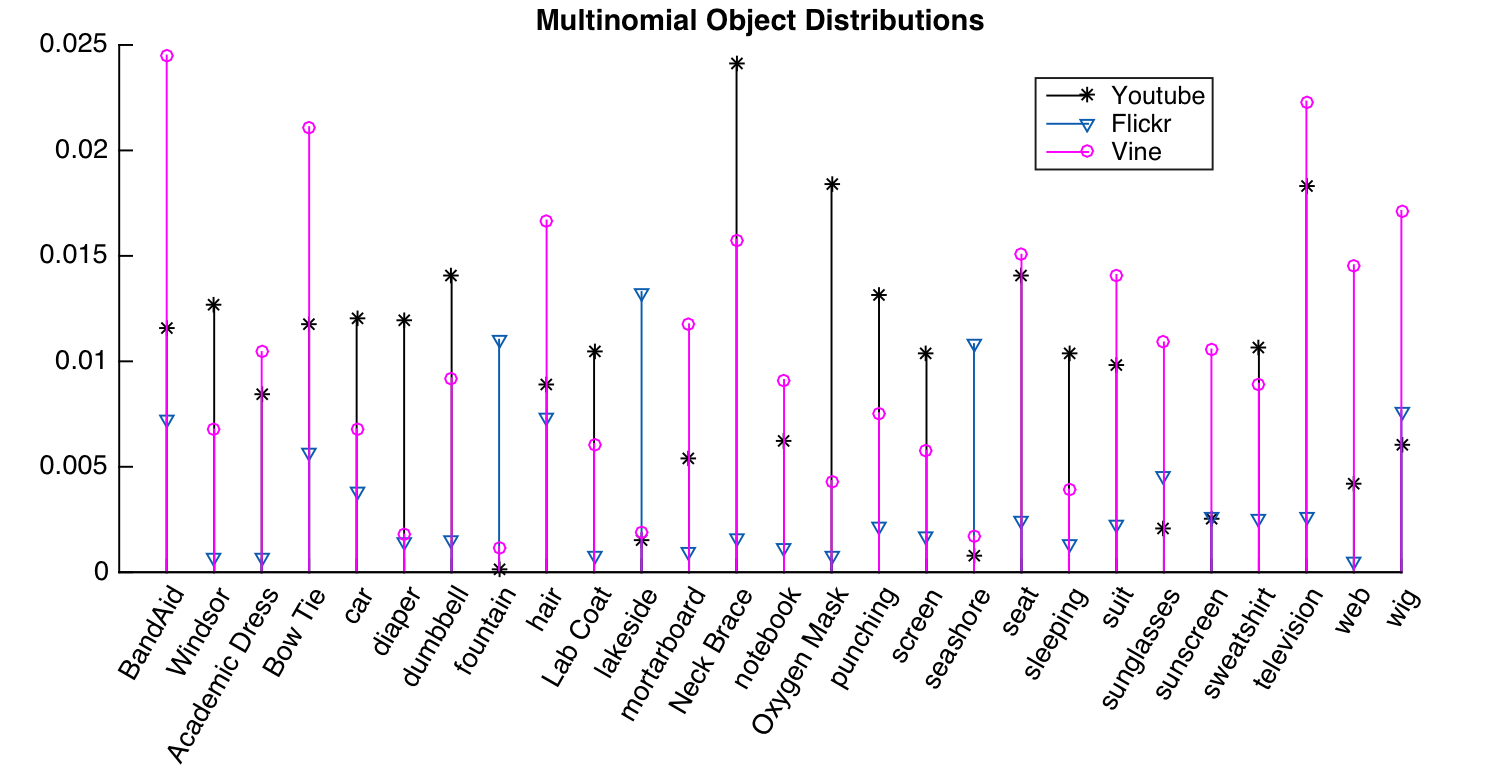
\includegraphics[width=\columnwidth]{plots/comparison/objects}
\caption{\textsl{ Distributions of the most distant object occurrences across platforms.}}
\label{fig:comparison_objects}
\end{figure}

\begin{figure}[!htb]
\centering
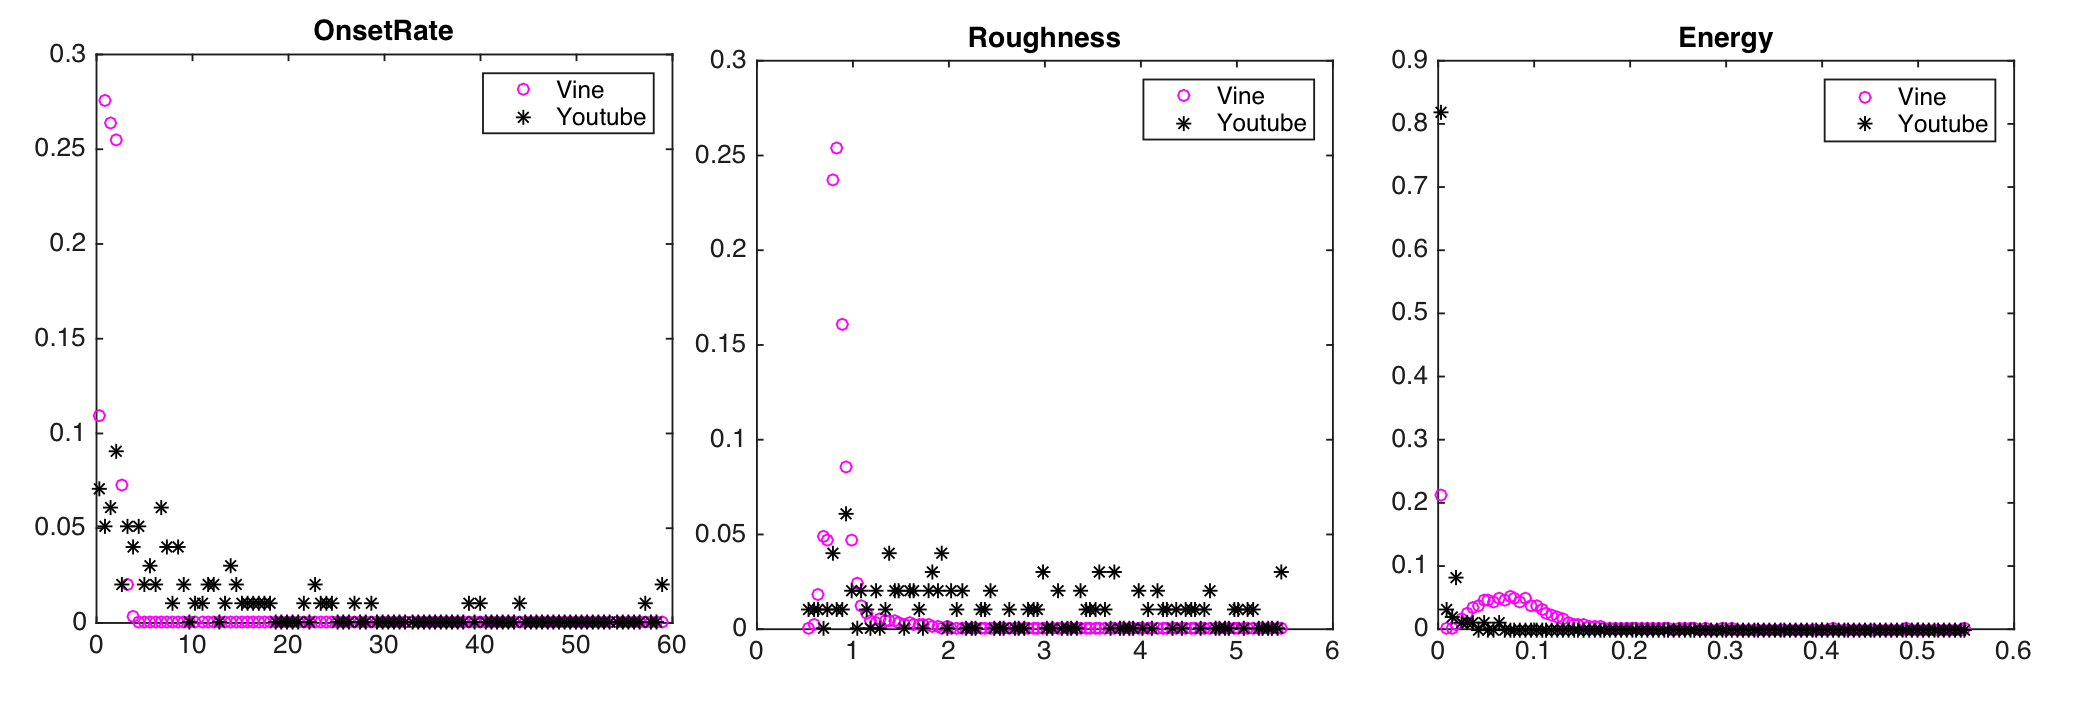
\includegraphics[width=\columnwidth]{plots/comparison/audio}
\caption{\textsl{ Distributions of the most diverging audio features across platformss.}}
\label{fig:comparison_audio}
\end{figure}
